\documentclass[twocolumn]{aastex62}

\newcommand{\vdag}{(v)^\dagger}
\newcommand\aastex{AAS\TeX}
\newcommand\latex{La\TeX}
\newcommand\s{$\sim$}
\newcommand{\e}{\'{e}}
\newcommand{\amen}[1]{\textbf{\textit{#1}}}

\usepackage{xcolor}

\shorttitle{From predictions to observation}
\shortauthors{Marian et al.}

\begin{document}

\def\lcdm{$\Lambda$CDM}
\def\hst{{\it HST}}
\def\efr{$R_{\mathrm{eff}}$}
\def\galfit{{\sc Galfit}}
\def\mbh{$\mathcal M_{\rm BH}$}
\def\lhost{$L_{\rm host}$}
\def\jcap{Journal of Cosmology and Astroparticle Physics}
\def\halpha{${\it H}\alpha$}
\def\hbeta{${\it H}\beta$}
\def\sersic{S\'ersic}
\def\lenstronomy{{\sc Lenstronomy}}
\def\Reff{{$R_{\mathrm{eff}}$}}
\def\kms{km~s$^{\rm -1}$}
\def\sigstar{{$\sigma_*$}}
\def\smass{{$M_*$}}
\newcommand{\Mgii}{Mg$_{\rm II}$}
\newcommand{\Civ}{C$_{\rm IV}$}

\title{From predictions to observation: scaling relations between supermassive black holes and their host galaxies at $1< z<2$}

\correspondingauthor{Xuheng Ding}
\email{dxh@astro.ucla.edu}

\author%[0000-0001-8917-2148]
{Xuheng Ding}
\affiliation{Department of Physics and Astronomy, University of California, Los Angeles, CA, 90095-
1547, USA}
\affiliation{School of Physics and Technology, Wuhan University, Wuhan 430072, China}

\author%[0000-0001-8917-2148]
{Tommaso True}
\affiliation{Department of Physics and Astronomy, University of California, Los Angeles, CA, 90095-
1547, USA}

\author%[0000-0001-8917-2148]
{John Silverman}
\affiliation{Kavli Institute for the Physics and Mathematics of the Universe, The University of Tokyo, Kashiwa, Japan 277-8583 (Kavli IPMU, WPI)}

\author{ET AL.}


\begin{abstract}
Recent observations have discovered the \mbh-host relation which are likely to be evolving as a function of redshift. This evolution trends are also emerged in the simulations. A direct comparison between the observation and simulation is important to help understand the insight of the their physical coupling and their growth. The simulating result would also help to correct the selection effect in the observation.
Here, we use the scaling relation using 32 X-ray-selected broad-line (type-1) AGN at $1.2 < z < 1.7$ and compare to the simulation. We decomposition the AGN image using state-of-art to infer the host luminosity and combining multi-band AGN luminosities to infer the stellar mass. We adopt the same selection function as the 32 AGNs to select two group of AGN samples from two state-of-the-art simulation projects, MassiveBlack-II (MBII) and semi-analytic models (SAMs). %MBII is the highest resolution simulation of this size which includes a self-consistent model for star formation, black hole accretion and associated feedback. The SAMs is ... 
We study the \mbh-\lhost and \mbh-\smass\ and find that simulating samples by the two simulations are well agree with the observations. Given that the relation of our high-z samples are offset to the local, we further track the histories of the simulating samples and investigate the origin of their relation and evolution. 
  
\end{abstract}

\keywords{keywords TBD}

\section{Introduction} \label{sec_intro}
The MBH-HOST relation by observation.

Introduce the mechanisms which could lead to this evolution.

In theory, the simulations have shown the similar trend, which could be a way to understand this relation and evolution.

In this work, we compare the observation to two state-of-the-art simulation projects. 


Throughout this paper, we adopt a standard concordance cosmology with $H_0= 70$ km s$^{-1}$ Mpc$^{-1}$, $\Omega{_m} = 0.30$, and $\Omega{_\Lambda} =
0.70$. Magnitudes are given in the AB system.

%\begin{figure*}[t]
%\centering
%\includegraphics[width = 18cm]{f01.pdf}
%\caption{Example of showing something.\textit{Left}: The some thing \textit{Right}: The some thing.}
%\label{fig:QSO_sample}
%\end{figure*}

\section{Comparison sample} \label{data}

\subsection{Observation data} 
We selected 32 new AGN systems from four X-ray coverage fields including COSMOS (Civano et al. 2016), (E)- CDFS-S (Lehmer et al. 2005; Xue et al. 2011), and SXDS (Ueda et al. 2008) at redshift range $1.2<z<1.7$. The X-ray selected sample have low nuclear-to-host ratios, which facilitates the extraction of the host properties. We adopt the \hst/WFC3 infrared channel to derive the high spatial resolution imaging data, to carry out the decomposition of the AGN-host using two-dimensional flux distribution. The details of the \hst\ observation and the study are presented in the companion paper. Moreover, 21/32 systems have \hst/ACS band, together with some other ground-based observations, which would provide the host information in the other bands. In the next section, we infer the reliable K-correction for the rest-frame R band luminosity and the SED to infer the stellar mass.

The \mbh\ of our sample have been estimated by \halpha\ and \hbeta\ in the FMOS survey. Comparing to the \Mgii\ and \Civ, the \mbh\ by broad Balmer lines are more trustworthy.
\textcolor{blue}{Do we need to list the \mbh\ and host properties in a table in this paper?}

\subsection{Simulating sample and the selection function} 
To compare with the observation, we adopt the sample from two state-of-the-art simulating projects, i.e., MassiveBlack-II (BHII) and ab-initio semi-analytic models (SAMs).

%Introduce BHII: The high resolution. In paper?, the simulation result shows that the evolution is exists since ... Some other interesting results.
The BHII is the highest resolution at the size of a comoving volume $V_{\rm box} = (100~{\rm Mpc}~h^{-1})$, including a self-consistent model for star formation, black hole accretion and associated feedback. The large simulation volume enable the simulating objects evolve independently; the high enough mass and spatial resolution meets the requirements for the object details. A variety of predictions by the simulation have been examined by comparing to the observations, including 
the Galaxy stellar mass function, quasar bolometric luminosity function (Khandai et al. 2015). %More recently, the simulated AGN systems 
%The simulating result:
The GSMF, The AGN bol luminosity; The M-Mstar relations. The AGNs compared to the observation (Aklant two papers).

%Introduce SAMs: Similarly, the simulation of SAMs shows that, the \mbh-host relation have stronger evidence in the bulge than disk...
On the theoretical side, aimed, high-resolution N-body simulations can study specific galaxy systems, but understanding the way of AGN feeding modes requires implementing the physics of nuclear gas inflows into cosmological models of galaxy formation. In turn, this requires an analytical description of such processes to be implemented into existing semi-analytic models.

We adopt a similar selection function to allow a comparing between equivalent samples. We plot the selection function of the observation data the the simulation data, in figure.
\begin{figure}[t]
\centering
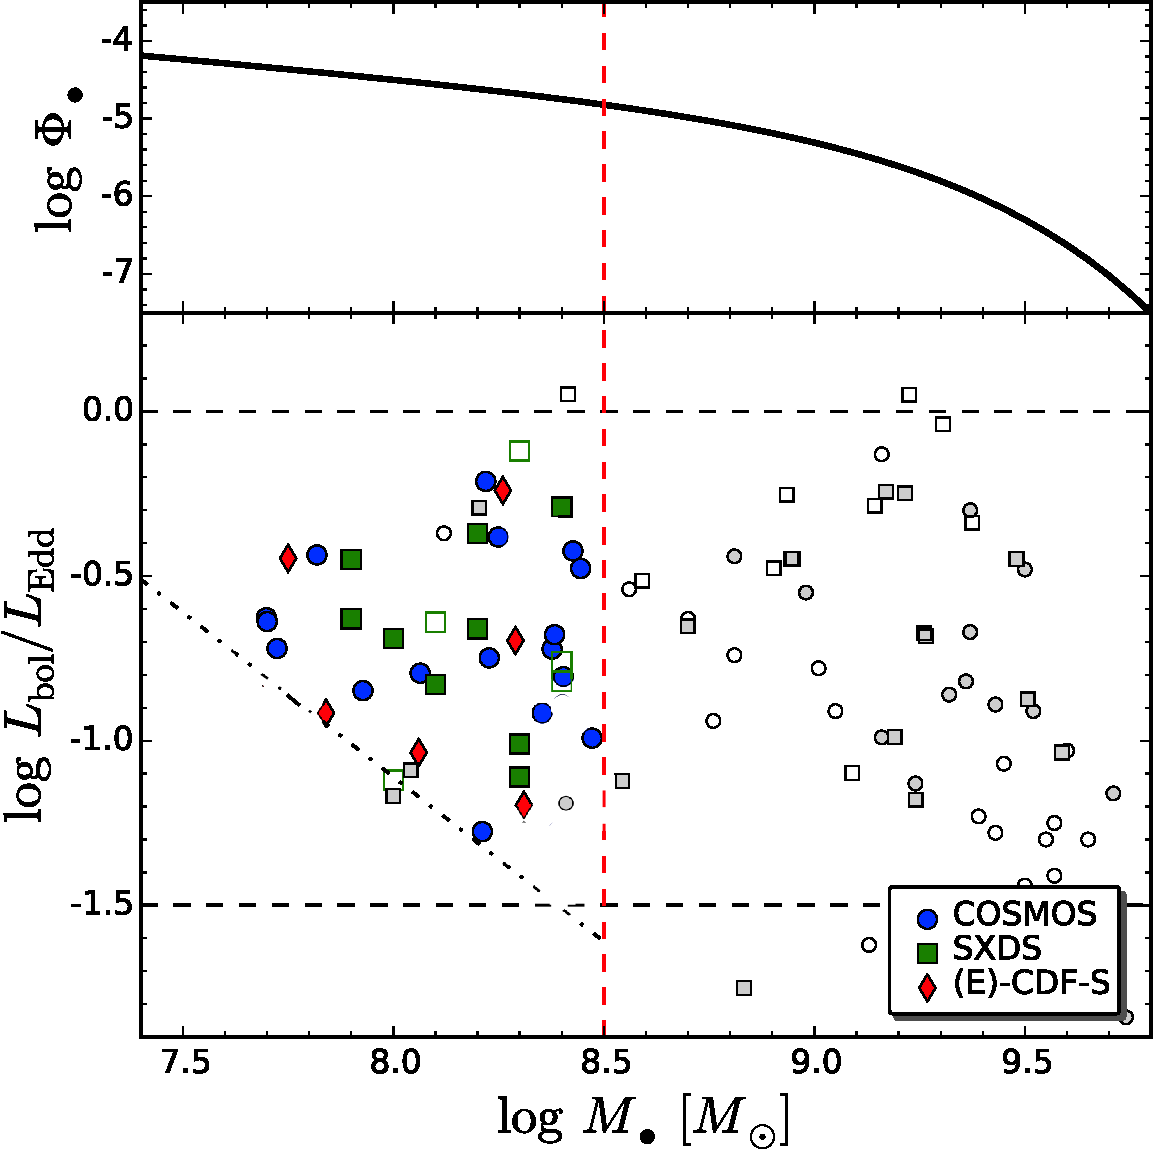
\includegraphics[width = 7cm]{hst_sample_bhmf_v8.pdf}
\caption{The selection function of our observation data.
Eddington ratios (LBol/LEdd) and BH masses (bottom panel) of our sample (in color) that fall well-below the knee of the BH mass function at z = 1.5 (top panel; Schulze et al. 2015). Dashed lines (vertical and horizontal) denote our selection window with the slanted line only shown to approximately illustrate the effect of a luminosity limit, inherent in the parent catalogs. For reference, we indicate the high-z luminous SDSS QSO samples (grey squares - Peng et al. 2006; grey circles - Decarli et al. 2010) with all falling above our chosen upper mass limit.
}
\label{fig:obs_selectfunc}
\end{figure}

\begin{figure}[t]
\centering
\includegraphics[width = 7cm]{BHII_selectfunc.pdf}
\caption{The sample selected from the BHII simulation.
}
\label{fig:bhII_selectfunc}
\end{figure}



\section{Result} 
\subsection{ML relation} 
1. The way to derive the MR magnitude.
2. Comparing the samples.

\begin{figure}[t]
\centering
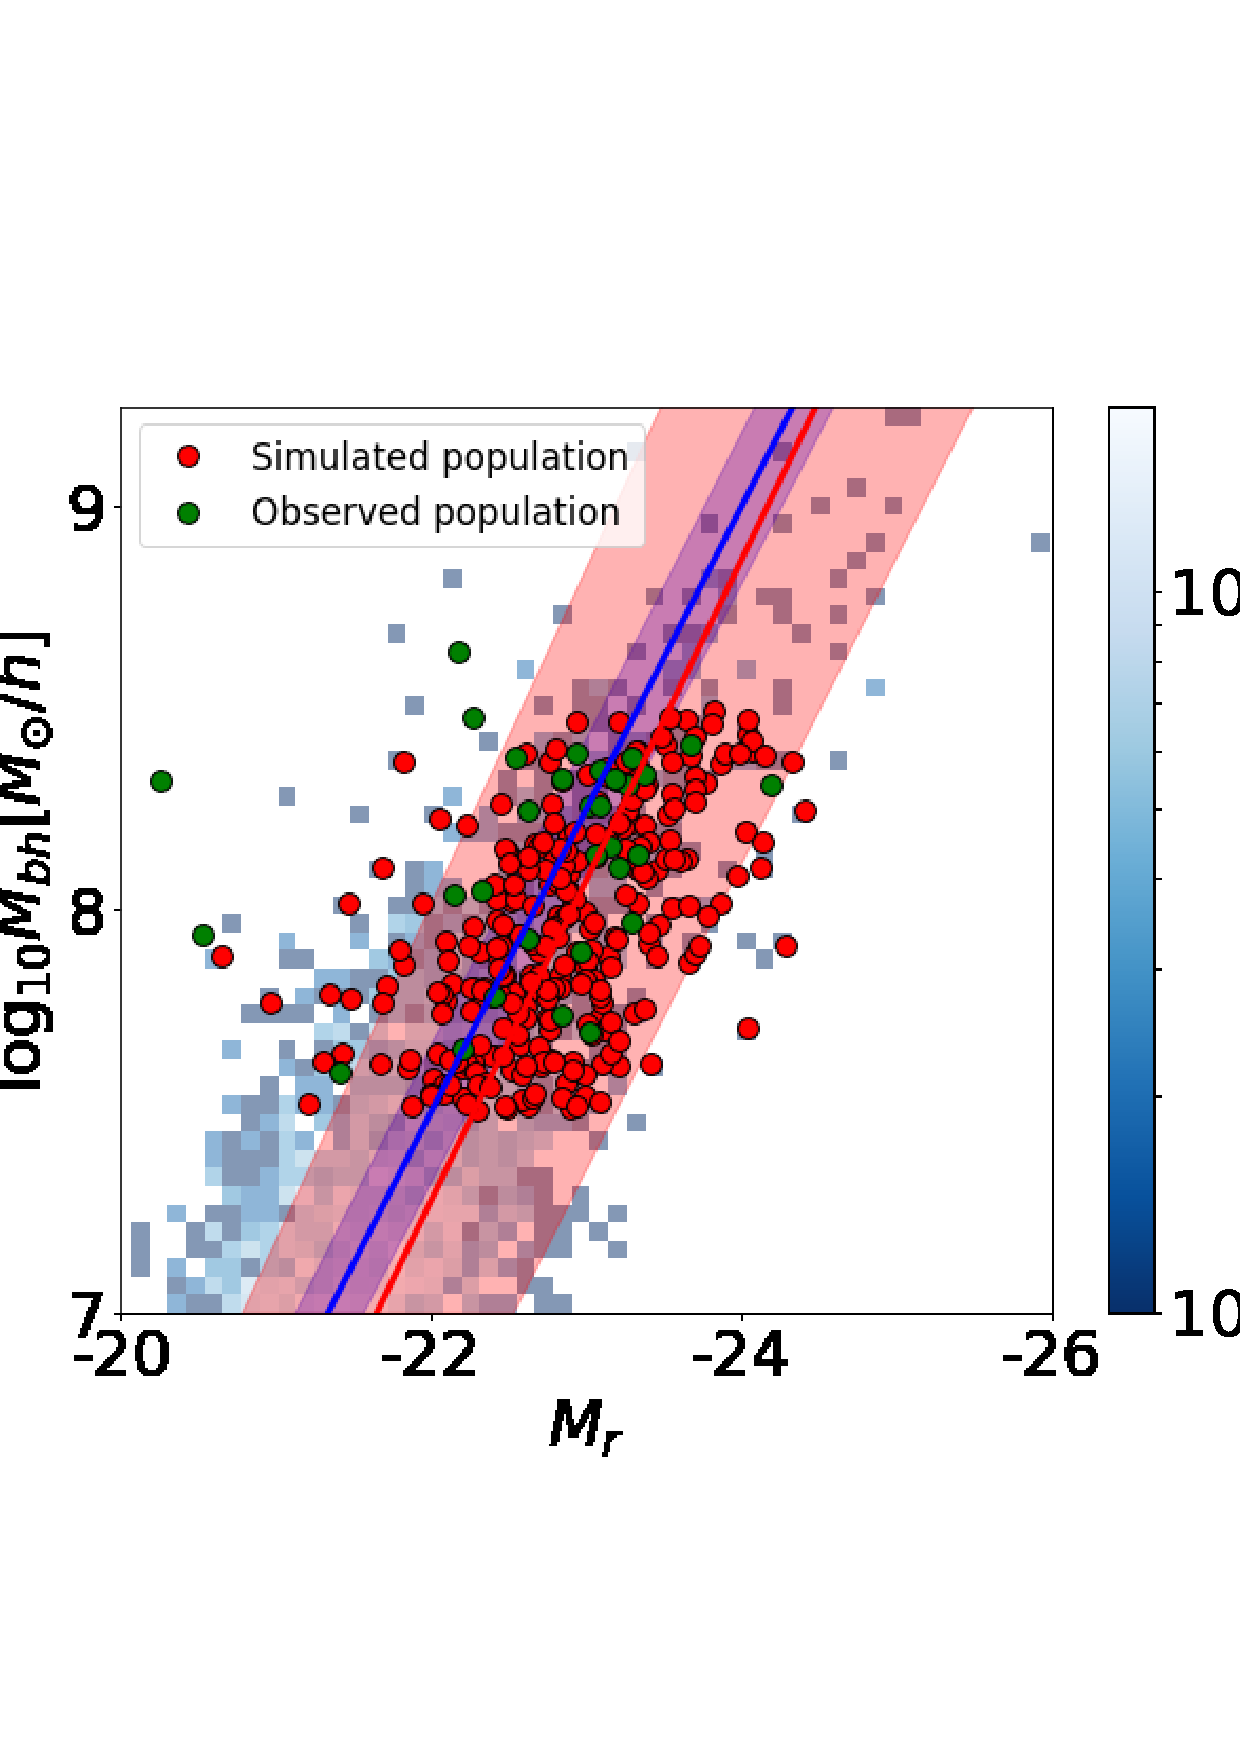
\includegraphics[width =  7cm]{BHII_ML.pdf}
\caption{M-L relation by BHII }
\label{fig:BHII_ML}
\end{figure}

\begin{figure}[t]
\centering
\includegraphics[width =  8cm]{SAM_ML.pdf}
\caption{M-L relation by SAM}
\label{fig:SAM_ML}
\end{figure}

\subsection{MM* relation} 
1. The SED to derive the Mstar.
2. Comparing the samples.


\begin{figure}[t]
\centering
\includegraphics[width =  8cm]{SAM_MMstar.pdf}
\caption{MMstar relation by SAM }
\label{fig:SAM_MM}
\end{figure}



\section{Summary \& Conclusions} \label{sec:summary}
We compared the inferred \mbh-host relations and compared with the simulations by 


\acknowledgments

X. Ding acknowledges support by China Postdoctoral Science Foundation Funded Project (No. 2017M622501).


\software{
        corner,
        Matplotlib \citep{matplotlib},
        }

\newpage

%\appendix

%\section{section}\label{appendix_section}
%TEXTTEXTTEXTTEXTTEXTTEXTTEXTTEXTTEXT
%\newpage

\bibliography{reference}
%\input{reference.bbl}

\end{document}